\chapter{Latent triple representations}\label{chap:embeddings}

\chapterQuote{\textit{``All problems in computer science can be solved by another level of indirection, except for the problem of too many layers of indirection.''}}{--- David Wheeler}

I dont like the name of this chapter, but I assume it was changed from Embeddings as to make it easier to non expert readers?

\chapterAbstract{E}{sta seccion habla de embeddings y como funcionan.
La que acabe estando en la version final de la tesis debe de ser bastante similar a la presentada x agu ya que el mundo de los embeddings no se ha movido mucho y se usan para practicamente lo mismo en ambas propuestas.}

Quizas moveria las prpuestas a una misma categoria mas general y pondria una tabla explicando los progesos de cada una de las ramas y luego entraria en detalles sobre las mas novedosas que hay ( y sobretodo en las que se han usado en el trabajo...)
% latent representation of a triple is one that exposes previously hidden knowledge, such as semantic similarity to some other triple. Obtaining such a representation is a popular way to perform Knowledge Graph completion, and it can be achieved in a number of ways. In this chapter we introduce the most prominent KG completion methods in the scientific literature that rely on latent representations. This chapter is structured in the following manner: Section~\ref{sec:emb-intro} provides an introduction to the matter, Section~\ref{sec:emb-tensors} presents the methods that perform  tensor factorization, Section~\ref{sec:emb-translations} introduces the models that are centered around embedded translations, Section~\ref{sec:emb-nn} discusses the number of ways in which neural networks can be used in this regard; finally, Section~\ref{sec:emb-summary} provides a summary of the contents of the chapter.

\section{Introduction}\label{sec:emb-intro}
que son y porque se usan en los grafos de conocimiento.

% A popular approach to Knowledge Graph completion consists on changing the representation medium of entities and relations entirely: instead of elements with a semantic meaning in a graph structure, they are represented in a numerical way. This then allows for the application of numerical methods to find missing entities, or missing connection between the existing entities. This is known as a latent representation.

% One such way is by using tensors, a mathematical structure that can hold data in any number of dimensions. Consequently, through a series of transformations, the original tensor representing the Knowledge Graph is turned into another that materializes some knowledge that was not previously readily available.

% Another popular latent representation is by creating an N-dimensional space and determining a position in it for every entity in a KG. An entity can then be referred to as the N-dimensional vector that represents its position. Such a space is known as an embedded space, and the position vectors are known as entity embeddings. In the embedded space, the plausibility of any given relation can be checked by performing a series of translations in it and evaluating the result, or by finding more complex relations between the entity embeddings thanks to the use of neural networks.

\section{Tensor factorization models}\label{sec:emb-tensors}
Rescal, SimplE, ComplEx etc etc...

% Tensors are a generalization of scalar numbers, vectors, matrices, and so on. Broadly, a tensor of order $N$ represents an $N$-dimensional collection of elements, where $N$ indices are necessary to address the position of an element. Any given Knowledge Graph can be represented using a third-order tensor of size $|E| \times |E| \times |R|$, namely $X = \{0, 1\}^{|E| \times |E| \times |R|}$, where $E$ is the set of entities in the KG, and $R$ is the set of possible relations in it. Using this representation, every element of the tensor is a binary number $\{0, 1\}$ denoting whether or not a given relation exists between a pair of entities. This concept is visually represented in Figure~\ref{fig:emb-kg2tensor}.

% \begin{figure}[!htp]
%     \centering
%     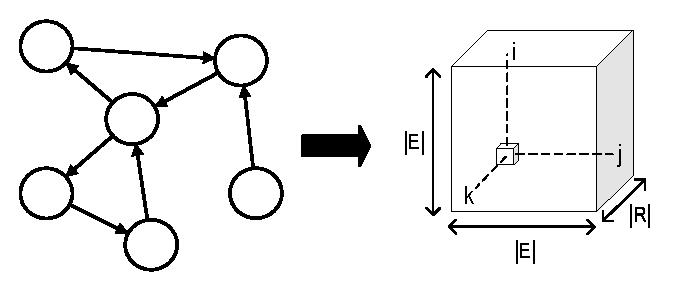
\includegraphics[width=.9\textwidth]{fig/embedding/kg2tensor}
%     \caption{Representing a KG as a third order tensor}
%     \label{fig:emb-kg2tensor}
% \end{figure}

% Once this representation is achieved, the goal of tensor factorization models is to compute a complementary tensor $Y = [0, 1]^{|E| \times |E| \times |R|}$ representing the correctness confidence of all possible combinations of entities and relations. Note that the elements in $X$ are binary, while those in $Y$ can take any real values between 0 and 1. Finally, to complete the KG, the facts with the highest confidences in $Y$ that are not still present in the Knowledge Graph are added into it.

% One of the first models in this line of work is RESCAL, which was proposed by \citet{nickel2011}. RESCAL represents the data in a Knowledge Graph using a tensor with the same structure as that shown in Figure~\ref{fig:emb-kg2tensor}. Then, it creates 2-dimensional slices of this tensor, one per each relation, which are illustrated in Figure~\ref{fig:emb-rescal}. Each slice, $X_r$, is factorized as $X_r = AB_{r}A^{T}$, where $A$ is a matrix that contains the latent representations of the entities, and $B$ is another matrix that represents the interactions of said entities for the relation $r$. Then, to predict the existence of a relation in them, the confidence scores are looked up in the computed latent representations.

% \begin{figure}[!htp]
%     \centering
%     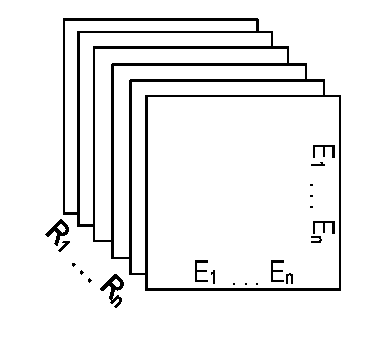
\includegraphics[width=.4\textwidth]{fig/embedding/sliced}
%     \caption{A third order tensor, sliced up in the RESCAL model}
%     \label{fig:emb-rescal}
% \end{figure}


% \citet{jenatton2012} proposed the LFM model, an extension of RESCAL that scales better to Knowledge Graphs with a higher number of relations. Similarly to the model it builds upon, LFM represents the tensor as a series of $X_r$ slices, but introduces a more complex factorization based on a bilinear structure that is able to capture one-, two-, and three-way interactions between the components of a triple. Additionally, the matrix that represents the interactions between the latent representations of the entities is further decomposed into smaller elements, which reduces the number of parameters required for its computation and thus increases the efficiency of the model.

% A combination of the previously discussed two approaches is proposed by \citet{garcia-duran2015}, who introduced the Tatec model. Tatec has features of both RESCAL and LFM, learning two different embedded representations of the same Knowledge Graph and combining their confidences together as $score(s, r ,t) = s_1(s, r, t) + s_2(s, r, t)$, where $(s, r ,t)$ can be any triple, and $s_1, s_2$ are the score functions of a bilinear and trilinear tensor factorization model, respectively. Naturally, the scores emitted by both models must be normalized before they can be combined. The authors also suggest and benchmark a series of possible alternative ways to combine the scores of the two constituent models within Tatec.

% \citet{liu2017} proposed the ANALOGY model, which is also an extension of RESCAL. ANALOGY derives its name from its focus on modelling and analyzing the analogical properties that are captured in the embedded representations of the entities. ANALOGY imposes further restrictions upon the relationship matrices of RESCAL, $B_r$, by demanding that they be normal ($B_rB_r^T = B_r^TB_r$) and commutative ($B_rB_{r'} = B_{r'}B_r$). This enables them to efficiently be block-diagonalized into a set of smaller matrices, which the authors show that enables them to be used in mathematical formulations of a lower complexity. Additionally, the factorization process of ANALOGY is guided by a fully-differentiable goal, which increases its computational scalability. 

% A similar effort was carried out by \citet{yang2014}, who introduced the DistMult model. The authors of DistMult propose replacing the dense $B_r$ matrix of the RESCAL model with a diagonal matrix, which greatly reduces its number of parameters and allows for a much speedier execution.

% \citet{tay2017} introduced the REST factorization model, which is especially tailored for large Knowledge Graphs. REST relies upon random walks to sample small subgraphs within the KG, and represents these subgraphs using tensors. The subgraphs are further split up using a relation sparsification technique, yielding even smaller tensors. The tensors representing different parts of the KG are combined together to produce an ensemble model that can be representative of the entire Knowledge Graph. This ensemble architecture is visually depicted in Figure~\ref{fig:emb-ensemble}. REST has provided satisfactory results in practice, and its ability to work on-demand make it a convenient choice for Knowledge Graphs that are in continuous expansion.

% \begin{figure}[!htp]
%     \centering
%     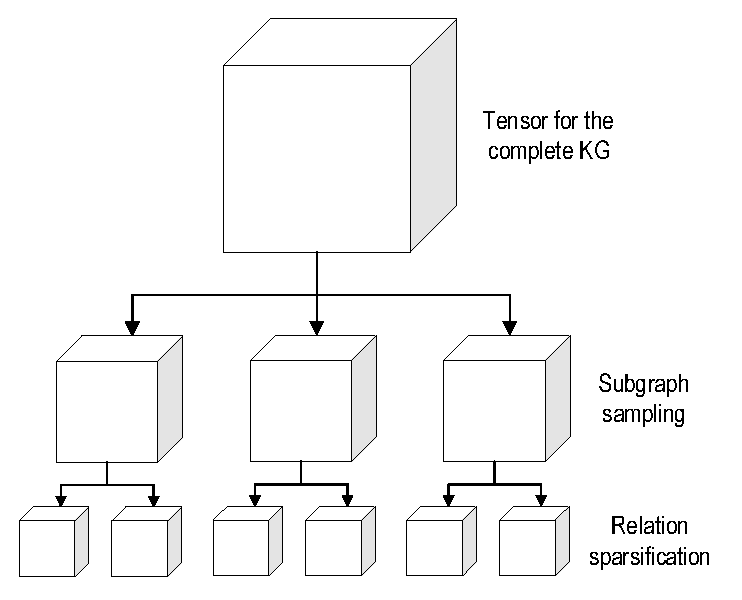
\includegraphics[width=.7\textwidth]{fig/embedding/ensemble}
%     \caption{An ensemble of tensors, as proposed by the REST model}
%     \label{fig:emb-ensemble}
% \end{figure}


% \citet{trouillon2016} proposed the ComplEx model, which is the first one to use complex instead of real values in the tensors. This can also be seen as splitting an embedded representation of the entities into two: one which contains the real values of the numbers, and one that contains the imaginary parts. This increases the expressiveness of the model, and makes it better suited to handle symmetric and antisymmetric relations, which are traditionally more challenging for the previously discussed models, due to the fact that they greatly increase the number of parameters they must deal with \cite{nickel2011, socher2013}. Perhaps counterintuitively, the use of complex numbers simplifies its score function, since it only uses the Hermitian dot product, which is the equivalent in $\mathbb{C}$ of the standard dot product in $\mathbb{R}$.\newpage

% Perhaps inspired by the naming of the previous model, \citet{kazemi2018} introduced the SimplE model, which aims to be more performant than other approaches in this category. For each relation $r$ present in a KG, SimplE considers an additional inverse relation $r^{-1}$ to it. Both are then represented using the vectors $v_r$ and $v_r^{-1}$, respectively. Thus, the confidence score for a triple $(s, r, t)$ is computed as the average of the confidence of $(s, r, t)$ and $(s, r^{-1}, t)$. This configuration allows the embedded representation of a relation and its inverse to be obtained independently, resulting in a higher expressivity and a good performance in practice.


\section{Translational models}\label{sec:emb-translations}

TransE, TransR y un muy larguisimo etc...

% A separate group of models represent entities as vectors in an N-dimensional space, called embeddings, and relations as translations in that space. From this starting point, their main goal is to define the transformations from entities to vectors and the translations in such a way that, for every triple $(s, r, t)$ in the KG, applying the translation defined by $r$ to the entity $s$ should result in a vector as close as possible to that of $t$. These models can then be used to provide a confidence value for the correctness of any triple, by evaluating to what extent this concept holds true.

% \citet{bordes2013} started this line of work with the TransE model. TransE defines a single N-dimensional space to which all entities in a KG are mapped, and in which every relation turns into a translation vector. Thus, it aims to generate this space in such a way that, for any given triple $(s, r, t)$, $v_s + v_r \approx v_t$, where $v_s, v_t$ are the vectors representing the $s$ and $t$ entities respectively, and $v_r$ represents the translation carried out by the relation $r$. The main intuition behind TransE is visually depicted in Figure~\ref{fig:emb-transE} for a simple 2D space.

% \begin{figure}[!htp]
%     \centering
%     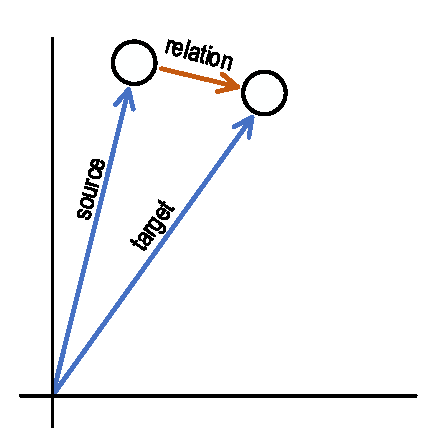
\includegraphics[width=.4\textwidth]{fig/embedding/transe}
%     \caption{Visual representation of the TransE model in a 2D space}
%     \label{fig:emb-transE}
% \end{figure}

% \citet{wang2014} proposed the TransH model, which improves TransE by considering that it may desirable for an entity to have a different embedded representation depending on the particular relation that is being considered. TransH achieves this by defining a particular hyperplane $w_r$ for every relation $r$, and then projecting the entities onto these planes as $e_\bot = v_e - w_r^{T}v_{e}w_r$, where $e$ can be any entity in the KG. Then, similarly to TransE, it optimizes the embedded space to ensure that $s_\bot + v_r \approx t_\bot$ for any triple $(s, r, t)$. A similar visual representation is provided in Figure~\ref{fig:emb-transH}.

% \begin{figure}[!htp]
%     \centering
%     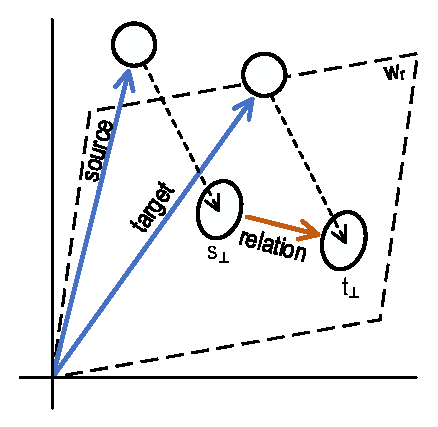
\includegraphics[width=.4\textwidth]{fig/embedding/transh}
%     \caption{Visual representation of the TransH model in a 2D space}
%     \label{fig:emb-transH}
% \end{figure}

% Following up with the previous idea, \citet{lin2015} proposed the TransR model. It acknowledges that an entity and a relation have a very different semantic meaning and, for this reason, TransR makes a twofold contribution. On the one hand, it defines two separate embedded spaces, one for entities and one for relations. On the other hand, it creates a different entity embedded space for each relation. The transition from the entity space to the relation space is performed through a relational projection matrix $M_r$. The translation goal thus becomes $v_sM_r + v_r \approx v_tM_r$. A graphical example of this is provided in Figure~\ref{fig:emb-transR}.

% \begin{figure}[!htp]
%     \centering
%     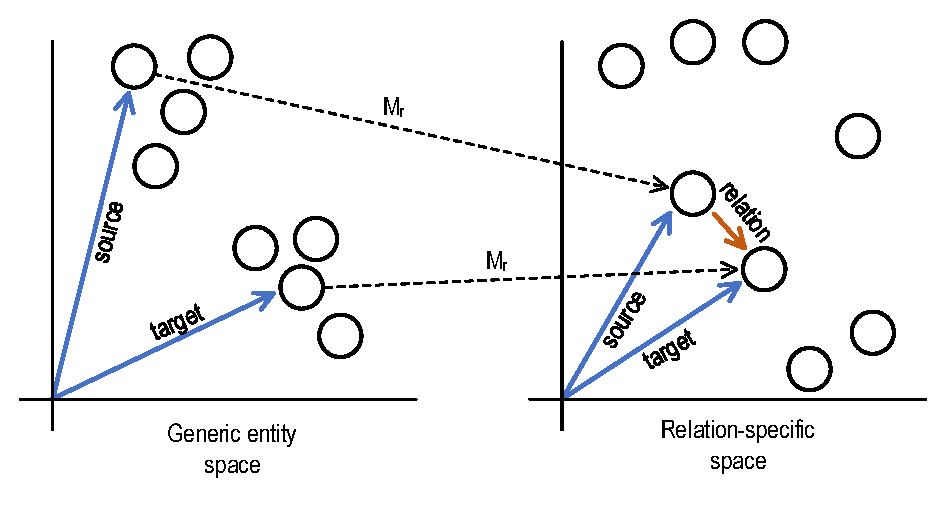
\includegraphics[width=.85\textwidth]{fig/embedding/transr}
%     \caption{Visual representation of the TransR model in a 2D space}
%     \label{fig:emb-transR}
% \end{figure}

% \citet{ji2015} introduced the TransD model, building upon TransH and improving it by constructing mapping matrices dynamically for every entity. Furthermore, it replaces the matrix multiplication operations used in the previous models with vector multiplications, which increases its operational speed. A similar approach is proposed by \citet{do2018} with TransF, which uses more lightweight matrices to perform the translation.

% \citet{fan2014} devised TransM, addressing the fact that the original TransE proposal considers all triples to be equally important, and thus they all contribute equally towards generating the embedded space in such a way that it optimizes the transformation goal. TransM adds a weight parameter that can be assigned to every individual triple, which affects its ability to influence the embedded space as a whole and acts as an attention mechanism.

% \citet{xiao2015} presented the TransA model, which uses an adaptive goal metric during the embedding generation process, overcoming the simple metrics used by other similar methods, making it more flexible when facing challenging relations.

% Perhaps facing the prospect of running out of letters in the English alphabet to continue with the previous naming scheme, \citet{sun2019} proposed the RotatE model, which defines an embedded space that uses complex numbers. Contrary to the previous models, where a translation is defined as a straight movement through the space, RotatE defines each relation as a rotation on the whole embedded space.

\section{Neural network-based models}\label{sec:emb-nn}
Como se aplican los embeddings a KG reasoning/completion. 

% In parallel to the development of research centered around Knowledge Graphs, the fields of neural networks (NNs) and deep neural networks (DNNs) have also seen significant improvements in the last decade \cite{vaswani2017, brown2020, rombach2022}.

% Consequently, a number of NN and DNN architectures have been applied to the problem of completing a Knowledge Graph, by virtue of transforming a triple into a representation that can be consumed by these models, and training them so that they can learn what constitutes correct knowledge. Contrary to the previously discussed translation-based models, NN models apply non-linear transformations to the data they are provided. This can result in an increased ability to deal with more complex data, however, it also makes their reasoning harder to understand.

% One of the first models that were proposed in this regard was NTN, by \citet{socher2013}. This model relies on a pre-computed set of word embeddings, in which semantically similar words are expected to be close to each other in the embedded space. NTN takes all the meaningful words in the name of an entity and averages the respective word embeddings together, resulting in a single embedding for every entity. In this manner, the embeddings of the two entities of a triple are provided as input to a bilinear neural network, which then outputs a confidence score for the entity pair. However, NTN is dependent on the availability and quality of the aforementioned word embeddings. Furthermore, these embeddings must be computed again if an entity with a novel word in its name is introduced in the Knowledge Graph. 

% A simplified version of NTN is used by \citet{dong2014} in their Multilayer Perceptron (MLP) proposal. MLP is used in the Google Knowledge Vault, a KG created by the same authors, to filter out possibly incorrect facts that are automatically extracted from plain text around the Web. To make it more lightweight in order to be applied to such a large KG, MLP changes the interaction function used by NTN to a multi-layer perceptron, which is much faster to train.

% A further refinement is proposed by \citet{liu2016}, who introduced the Neural Association Model (NAM). It uses deep neural networks to learn and infer the joint conditional probabilities between two facts. One of the main strengths of NAM is its increased explainability, since using conditional probabilities makes it easier to justify the correctness of a triple using other triples known to be correct as supporting evidence.

% \citet{guan2018} proposed a Shared Embedding-based neural network (SENN) for the task of KG completion. SENN aims to achieve a higher level of specialization by using three separate neural sub-structures to predict a missing source entity, relation, or target entity in a triple. The results of these structures are combined together to assess the correctness of a whole triple. By virtue of being an ensemble of smaller structures, SENN is also more efficient than some of the other pre-dating models.

% The interconnected nature of Knowledge Graphs also calls for the application of convolutional neural networks (CNNs). These networks do not focus on only one entity at a time; they are also able to derive information from other entities close to it, having a larger picture of the KG as a whole. In this line, \citet{dettmers2018} introduced ConvE, a two-dimensional CNN that operates on the entire matrix that represents entity embeddings. ConvE uses a traditional 2D convolution to augment its predictive capabilities with respect to more classical NN architectures. It also has a more reduced number of parameters that must be trained, increasing its efficiency.

% An evolution of ConvE is the InteractE model, proposed by \citet{vashishth2020}. InteractE uses a novel circular convolutional structure, which enables it to capture more meaningful interactions. \citet{nguyen2019} also build upon the main idea of ConvE to introduce CapsE, a method that works by using a capsule network \cite{sabour2017} that converts the entities of a Knowledge Graph into images, and then performing more traditional 2D convolutions on said images.

% In more recent years, graph convolutional networks, also called simply graph neural networks (GNNs) have emerged as a way to apply NNs to graph-like structures \cite{bruna2014, wu2021, zhou2020, kipf2017}. It seems thus reasonable that Knowledge Graph completion could benefit from the application of GNNs \cite{ye2022}. %Recently, \citet{TODO fernando} have studied the application of GNNs to KG completion and other related tasks, reaching the conclusion that they can generally outperform traditional neural networks, although more work and fine-tuning is needed to achieve consistent results.

% In this regard, \citet{schlichtkrull2018} proposed R-GCN, a type of GNN that leverages graph neighborhoods in order to complete them. \citet{shang2019} have proposed SACN, an encoder-decoder method based on this type of NN. For encoding, SACN uses a composition of multiple weighted GNNs that is able to leverage information from the structure of a Knowledge Graph and the attributes contained in its entities. The decoder uses a modified version of the previously mentioned ConvE model. The addition of GNNs allows it to outperform the original ConvE method.

\section{Summary}\label{sec:emb-summary}
% In this chapter, we have presented an overview of the existing methods for Knowledge Graph completion in the literature that rely on latent triple representations. We have introduced and described the models that use tensors to model a KG, and then factorize those tensors to obtain a predictive model. We have also presented the models that embed entities in a higher-order space and perform translations on them to find missing knowledge. Finally, we have enumerated the methods that use neural networks to perform Knowledge Graph completion, and we have presented the neural network architectures that are commonly used for this task.

brief summary of all the facts presented.